
\documentclass[twoside]{report}
%[a4paper,twoside,openright]
% Twoside implica che i capitoli inizino sempre con la prima pagina a sinistra, eventualmente lasciando una pagina vuota nel capitolo precedente. 

\usepackage{tcolorbox}
% Blue Quotebox
\newtcolorbox[auto counter, number within=section]{quotebox}[2][]{colframe=black, colback=white, 
coltitle=black, fonttitle=\bfseries, arc=1mm, 
before=\vskip\baselineskip, 
left=2pt, % This adds the vertical line
title={#2},#1
}

% Yellow Quotebox
\newtcolorbox[auto counter, number within=section]{quotebox-yellow}[2][]{%
    colframe=yellow!80!black, % Border color (dark yellow)
    colback=yellow!20,        % Background color (light yellow)
    coltitle=black, % Title color
    fonttitle=\bfseries,      % Title font
    arc=1mm,                  % Rounded corners
    before=\vskip\baselineskip, % Vertical space before the box
    left=2pt,                 % Vertical line spacing
    title={#2},#1             % Title handling
}

% Grey Quotebox
\newtcolorbox[auto counter, number within=section]{quotebox-grey}[2][]{%
    colframe=gray!50,       % Border color
    colback=gray!5,     % Background color (light grey)
    coltitle=black,      % Title color
    fonttitle=\bfseries, % Title font
    arc=1mm,             % Rounded corners
    before=\vskip\baselineskip, % Vertical space before the box
    left=2pt,            % Vertical line spacing
    title={#2},#1        % Title handling
}

% Red Quotebox
\newtcolorbox[auto counter, number within=section]{quotebox-red}[2][]{%
    colframe=red!50!black!75,   % Slightly darker red border for better contrast
    colback=red!5,          % Light red/pink background
    coltitle=black,          % Title text color set to black
    fonttitle=\bfseries,     % Title font
    arc=1mm,                 % Rounded corners
    before=\vskip\baselineskip, % Vertical space before the box
    left=2pt,                % Vertical line spacing
    title={#2},#1            % Title handling
}

%prova
\usepackage[utf8]{inputenc} % For UTF-8 support
\usepackage{mdframed} % For the vertical line on the left
% Define a custom style for the vertical line
\newmdenv[
    topline=false, % No top border
    bottomline=false, % No bottom border
    rightline=false, % No right border
    leftline=true, % Only left border
    linecolor=black, % Black line color
    linewidth=1pt, % Thickness of the left line
    innerleftmargin=5pt, % Space between the line and the text
    innerrightmargin=0pt, % No right margin
    innertopmargin=0pt, % No top margin
    innerbottommargin=0pt % No bottom margin
]{customquote}
%--------------------
\usepackage{xcolor}

% Dimensione dei margini
\usepackage[a4paper,top=2cm,bottom=1.5cm,left=1.5cm,right=1.5cm]{geometry} 
% Dimensione del font
\usepackage[fontsize=9pt]{scrextend}
% Lingua del testo
\usepackage[english]{babel}
% Lingua per la bibliografia
\usepackage[fixlanguage]{babelbib}
% Codifica del testo
\usepackage[utf8]{inputenc} 
% Encoding del testo
\usepackage[T1]{fontenc}
% Per modificare l'header delle pagine 
\usepackage{fancyhdr}               

\usepackage{float}

% Librerie matematiche
\usepackage{amssymb}
\usepackage{amsmath}
\usepackage{amsthm}         

% Uso delle immagini
\usepackage{graphicx}
% Uso dei colori
\usepackage[dvipsnames]{xcolor}         
% Uso dei listing per il codice
\usepackage{listings}          
% Per inserire gli hyperlinks tra i vari elementi del testo 
\usepackage{hyperref}     
% Diversi tipi di sottolineature
\usepackage[normalem]{ulem}
%to divide content into colums
\usepackage{multicol}
% -----------------------------------------------------------------

% Modifica lo stile dell'header
\pagestyle{fancy}
\fancyhf{}
\lhead{\rightmark}
\rhead{\textbf{\thepage}}
\fancyfoot{}
\setlength{\headheight}{16pt}

% Rimuove il numero di pagina all'inizio dei capitoli
\fancypagestyle{plain}{
  \fancyfoot{}
  \fancyhead{}
  \renewcommand{\headrulewidth}{0pt}
}

\definecolor{backcolour}{rgb}{0.90,0.95,0.92}
\definecolor{Light blue}{rgb}{173,216,230}
% Stile del codice
% \lstset{style=codeStyle}
\lstdefinestyle{codeStyle}{
    backgroundcolor=\color{backcolour},
    commentstyle=\color{teal},
    keywordstyle=\color{Magenta},
    numberstyle=\tiny\color{gray},
    stringstyle=\color{violet},
    basicstyle=\ttfamily\scriptsize,
    breakatwhitespace=false,     
    breaklines=true,                 
    captionpos=b,                    
    keepspaces=true,                 
    numbers=left,                    
    numbersep=5pt,                  
    showspaces=false,                
    showstringspaces=false,
    showtabs=false,
    tabsize=1
} \lstset{style=codeStyle}

% \lstset{style=longBlock}
\lstdefinestyle{longBlock}{
    commentstyle=\color{teal},
    keywordstyle=\color{Magenta},
    numberstyle=\tiny\color{gray},
    stringstyle=\color{violet},
    basicstyle=\ttfamily\scriptsize,
    breakatwhitespace=false,         
    breaklines=true,                 
    captionpos=b,                    
    keepspaces=true,                 
    numbers=left,                    
    numbersep=5pt,                  
    showspaces=false,                
    showstringspaces=false,
    showtabs=false,                  
    tabsize=2
} \lstset{style=codeStyle}

% Togliendo il commento al comando che segue, si inseriscono nella bibliografia anche le fonti presenti in Bibliography.bib ma non citati direttamente con il comando \cite
\nocite{*}

% Margini prima e dopo blocchi di codice, per avere più distanza
\lstset{aboveskip=20pt,belowskip=20pt}

% Modifica dello stile dei riferimenti
\hypersetup{
    colorlinks,
    linkcolor=black,
    citecolor=black
}

% Aggiunti definizioni, teoremi, linea e listing
\newtheorem{definition}{Definizione}[section]
\newtheorem{theorem}{Teorema}[section]
\providecommand*\definitionautorefname{Definizione}
\providecommand*\theoremautorefname{Teorema}
\providecommand*{\listingautorefname}{Listing}
\providecommand*\lstnumberautorefname{Linea}

\raggedbottom
\usepackage{graphicx} % Required for inserting images

\title{Information systems security}
\author{Lorenzo Di Maio}
\date{October 2024}

\begin{document}

\maketitle
\tableofcontents
%There we have to insert the chapters
\chapter{Authentication techiniques protocols, and architecures}

Authentication refers to the process of verifying the identity of an entity (whether it's a human, software component, or hardware element) 
before granting access to resources in a system. Authentication can be applied to various type of "actors", such as:
\begin{itemize}
    \item \textbf{Human being}
    \item \textbf{software component}
    \item \textbf{Hardware element}
\end{itemize}

\subsubsection{Authentication vs Authorization}
\begin{itemize}
    \item \textbf{Authentication (authC/authN)}: established the indetity of an entity.
    \item \textbf{Authorization (authZ)}: determines where a authenticated entity has permission to access.
\end{itemize}

\section{Authentication factors}
Authentication can be based on 3 primary factors:
\begin{itemize}
    \item \textbf{Knowledge}: Information that only the user knows and can provides as proof of ther identity.
    \item \textbf{Ownership}: Physical object or device that only the user has access to.
    \item \textbf{Inherence}: This factor relies on onique biological traits of the user (e.g fingerprint).
\end{itemize}
\textbf{N.B.} Authentication can be applied not just to human user, but also to processes and devices.

\subsection{Risks}
\begin{itemize}
    \item \textbf{Knowledge:}
    \begin{itemize}
        \item \underline{Storage} \(\rightarrow \) if passwords are stored improperly, they are vulnerable to thieft. 
        \item \underline{Demonstration} \(\rightarrow\) user might inadvertently reveal their password through social engineering.
        \item \underline{Transmission} \(\rightarrow\) if passwords are sent over ensecured channel, they can be intercepted by attackers. 
    \end{itemize}
    \item \textbf{Ownership:}
    \begin{itemize}
        \item \underline{Authentication thieft}
        \item \underline{Cloning}
        \item \underline{Unathorized usage}
    \end{itemize}
    \item \textbf{Inherence:}
    \begin{itemize}
        \item \underline{Counterfeiting} \(\rightarrow\) biometric data can be spoofed or replicated by attackers using sophisticated techiniques.
        \item \underline{Privacy} \(\rightarrow\) the use of biometric data riases the risk of biometric information being exposed.
        \item \underline{Irreversibility} \(\rightarrow\) biometric traits cannot be raplaced if compromised. 
    \end{itemize}
\end{itemize}

\section{Digital Authentication model (NIST SP800.63B)}
\begin{figure}[h]
    \centering
    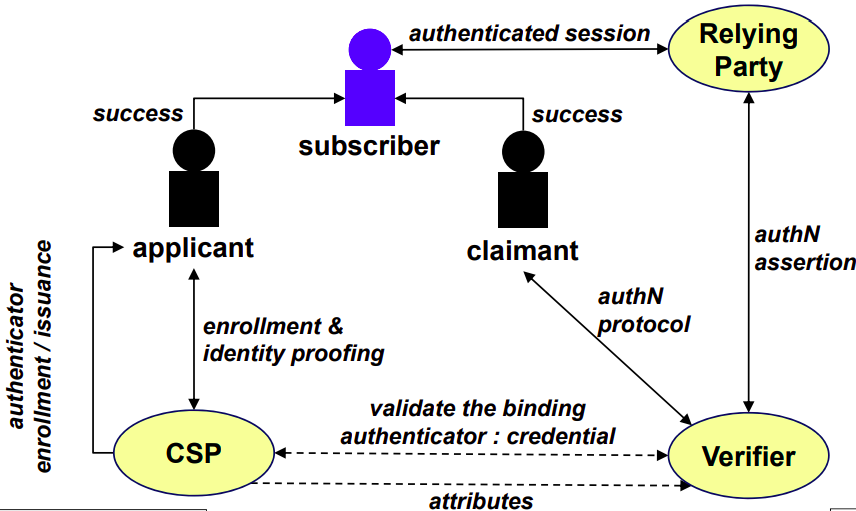
\includegraphics[width=0.5\textwidth]{/home/lorenzo/Notes/Information System Security/images/Screenshot from 2024-11-13 20-29-06.png}
\end{figure}
\textbf{Entities:}
\begin{itemize}
    \item \textbf{Subscriber}: appliacant who has succesfully completed identity proofing.
    \item \textbf{Appliacant}: an indiviual applying to established a digital identity.
    \item \textbf{Claimant}: the user trying to prove their identity to access a system or service.
    \item \textbf{Relying Party}: will request/receive an authN assertion from the verifier to asses user identity (and attributes).
    \item \textbf{Verifier}: validates the user's credential during each authentication event. 
    \item \textbf{CSP}: 
        \begin{itemize}
            \item Verifies the applicant's indetity during the initial enrollment process. 
            \item Issue a credential and bines it to an authenticator for the user.
        \end{itemize} 
\end{itemize}


\section{Generic authentication protocol}
\begin{minipage}{0.5\textwidth}
    \begin{enumerate}
        \item The user initiates an authentication request by sending their UID.
        \item The user generates a proof based on their secret, useing a secure function \(F(S_{UID})\), and send this proof to the verifier.
        \item The verifier checks if the received proof matches the stored representation of the secret.
        \item If it matches, the user is succesfully authenticated.
    \end{enumerate}
\end{minipage} 
\hspace{1cm}
\begin{minipage}{0.5\textwidth}
    \centering
    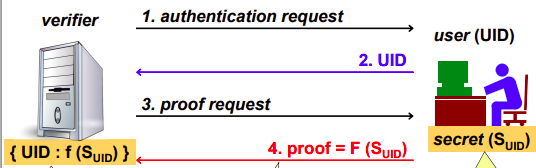
\includegraphics[width=\textwidth]{/home/lorenzo/Notes/Information System Security/images/Screenshot from 2024-11-14 11-06-55.png}
\end{minipage}



\section{Password base authentication}
\begin{minipage}{0.5\textwidth}
    \begin{enumerate}
        \item The user sends their UID and \(P_{UID}\) (= Password) to the verifier.
        \item The server verifies the proof:
        \begin{itemize}
            \item If password are stored in cleartext, it directly compares the proof with the stored password.
            \item If password are stored in hashes, it hasesh the proof and compares it to the store hash \(H_{UID}\).
        \end{itemize}
    \end{enumerate}
\end{minipage} 
\hspace{1cm}
\begin{minipage}{0.5\textwidth}
    \centering
    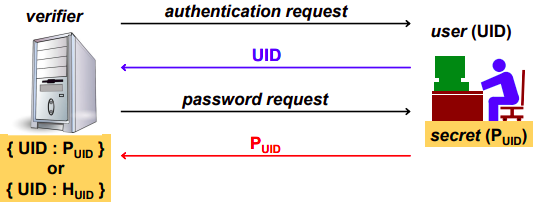
\includegraphics[width=\textwidth]{/home/lorenzo/Notes/Information System Security/images/Screenshot from 2024-11-14 11-09-10.png}
\end{minipage}

\begin{quotebox}[colframe=blue!10!white, colback=blue!5!white]{Problems of reusable Passowrds}
    \begin{itemize}
        \item \textbf{PWD Sniffing} (attackers intercept password during transmission)
        \item \textbf{PWD Database attack} (if DB contains plaintext or obfuscated PWD)
        \item \textbf{PWD Guessing} (very dangerous if it can be done offline, e.g against a list of PWD hashes)
        \item \textbf{PWD Enumeration} (PWD brute force attack)
        \begin{itemize}
            \item If PWD is limited in lenght and/or character type.
            \item If authN protocol does not block repeated failures.
        \end{itemize}
        \item \textbf{PWD Duplications} (using the same PWD for one service against another one, due to user PWD reuse)
        \item \textbf{Crypographic Aging} (as computing power grows, older crypographic methods become vulnerable to new attacks)
        \item \textbf{PWD capture via server spoofing and phishing} (attackers deceive user into givining away their PWD by pretending to be legitimate service)
    \end{itemize} 
\end{quotebox}

\begin{quotebox}[colframe=blue!10!white, colback=blue!5!white]{Password best practies}
    Suggestion to reduce password risks:
    \begin{itemize}
        \item Use alphabetical characters (upper case + lower case), digits and special characters
        \item Make passwords long (at least 8 character)
        \item Never use dictionary words
        \item Change password regularly, but not too frequently
        \item Do not reuse passwords across different services
    \end{itemize}
\end{quotebox}


\begin{quotebox}[colframe=blue!10!white, colback=blue!5!white]{Password storage}
    \begin{itemize}
        \item \textbf{Server Side:}
        \begin{itemize}
            \item Passwords should never be stored in cleartext.
            \item \underline{Encrypted passwords} aren't ideal since the server would need to know the encryption key.
            \item \underline{Better to store a password digest} (hashed password), though vulnerable to dictionary attacks.
            \item \underline{Rainbow tables} can speed up these attacks, so it’s important to add a “salt” (random variation) to each password.
        \end{itemize}
        \item \textbf{Client-side:}
        \begin{itemize}
            \item Ideally, passwords are memorized by the user, but having many passwords makes this difficult.
            \item People may resort to writing them down or using simple passwords, which is risky.
            \item \underline{Using a password manager} or encrypted file is a safer alternative.
        \end{itemize}
    \end{itemize}
\end{quotebox}


\section{The "dictionary" attack}
\begin{itemize}
    \item \textbf{Hypothesis:} The attacker knows the hash algorithm and the hashed password values.
    \item \textbf{Pre-computation:} For each word in a dictionary, compute and store its hash \(store(DB,Word,hash(World))\)
    \item \textbf{Attack process:}
    \begin{itemize}
        \item Let \(HP\) (=hash password) to be the hash of an unknown password.
        \item Lookup \(HP\) in the precomputed dictionary \((DB)\) to find a matching password.
        \item If found, output the password; if not, indicate it's "not in dictionary".
    \end{itemize}
\end{itemize}

\section{Rainbow Table attack}
Rainbow Table is a \textbf{space-time trade-off technique} that reduces storage needs for exhaustive hash tables, making certain brute-force attacks feasible within limited space.
It uses a reduction function \(r:h \rightarrow p\) (which is NOT \(h^{-1}\)) to generate chains of hashes.
\\ \textbf{Example:}
\begin{itemize}
    \item For a 12-digit password, an exhaustive hash table woudl require \(10^{12}rows(P_i:HP_i)\) 
    \item rainbow = \(10^9\) rows, each representing 1000 possible passwords.
\end{itemize}

\begin{center}
\begin{minipage}{0.5\textwidth}
    \begin{quotebox}[colframe=blue!10!white, colback=blue!5!white]{Attack}
        \centering
        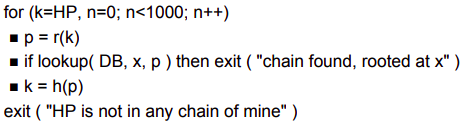
\includegraphics[width=0.8\textwidth]{/home/lorenzo/Notes/Information System Security/images/Screenshot from 2024-11-14 11-51-24.png}
\end{quotebox}
\end{minipage}
\end{center}

\section{Salting Passwords: A Defense Against Dictionary and Rainbow Table Attacks}
\textbf{Salting passwords} is a security technique used to protect stored passwords from dictionary attacks and rainbow table attacks. A salt is a unique, random string added to each password before hashing. This ensures that even if two users have the same password, their hashes will be different due to the unique salt.
\newline
\newline
\begin{minipage}[t]{0.5\textwidth}
    \subsubsection{Steps for each user (UID):}
    \begin{itemize}
        \item Generate or ask for the user's password.
        \item Create a unique, random slat for each user.
        \item Compute the salted hash:\(SHP=hash(password\ ||\ salt)\)
        \item Store the triplet \(\{UID,\ SHP,\ salt\}\)
    \end{itemize}
\end{minipage} 
\hspace{0.5cm}
\begin{minipage}[t]{0.5\textwidth}
    \subsubsection{Password Verification with Salt}
   \begin{itemize}
    \item \textbf{Claimant:} Provides their user ID (UID) and password (PWD).
    \item \textbf{verifier:} 
    \begin{itemize}
        \item Uses the UID to find the stored salted hash (SHP) and salt. 
        \item Computues \(SHP'=hash(PWD\ || \ salt)\).
    \end{itemize}
   \end{itemize}
\end{minipage}
\begin{quotebox}[colframe=blue!10!white, colback=blue!5!white]{The Linkedin attack}
In 2012, LinkedIn was breached, exposing 6.5 million unsalted SHA-1 password hashes. The lack of salting allowed attackers to crack at least 236,578 passwords through crowdsourced efforts before restrictions halted the exposure.
\end{quotebox}

\noindent\rule{1\textwidth}{0.00001pt}

\section{Strong authentication definitions}
The concept of strong authentication (authN) is crucial in ensuring secure identity verification, but it has never been formally defined with a universal definition.
Various definitions exist depending on the context, such as the European Central Bank (ECB) and PCI-DSS.

\begin{quotebox}[colframe=blue!10!white, colback=blue!5!white]{ECB definition}
    The ECB defines strong authentication as a process that involves at least two independent 
    elements from \textbf{knowledge} (e.g. password), \textbf{ownership} (e.g. smartcard), 
    and \textbf{inherence} (e.g. biometrics). The key requirement is that these elements 
    must be mutually independent, so compromising one should not affect the others. 
    Furthermore, at least one element should be \textbf{non-reusable} or \textbf{non-replicable} 
    (except for inherence), with the entire process safeguarding the confidentiality of the 
    authentication data.
\end{quotebox}

\begin{quotebox}[colframe=blue!10!white, colback=blue!5!white]{PCI-DSS Definition}
    PCI-DSS mandates \textbf{multi-factor authentication (MFA)} for access to cardholder data, 
    particularly for administrators and remote access from untrusted networks. Since version 3.2, MFA has become compulsory for remote access, 
    and the use of the same factor twice (e.g., two passwords) does not qualify as MFA.
\end{quotebox}

\section{Challenge-Response Authentication (CRA)}
Challenge-response authentication (CRA) is a widely used technique where 
a challenge is issued, and the claimant responds by solving it with a 
secret (shared or private). The challenge must be \textbf{non-repeatable} 
(usually a random nonce) to avoid replay attacks. The function used to compute 
the response must be \textbf{non-invertible}, otherwise, a listener can record the 
traffic and easily find the shared secret:
\[ if(\exists f^{-1})\ then\ K_c\ =\ f^{-1}(response, challenge)\]

\subsection{Symmetric CRA}
\begin{minipage}{0.3\textwidth}
    \vspace{-0.9cm}
    Symmetric CRA involves a shared secret (like a password or key) between 
    the claimant and verifier. This method is fast, often utilizing hash 
    functions (e.g., SHA1, SHA2, SHA3).
\end{minipage} 
\hspace{0.001cm}
\begin{minipage}{0.7\textwidth}
    \centering
    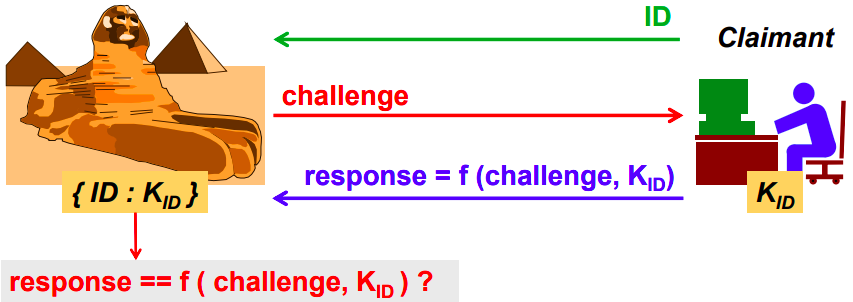
\includegraphics[width=0.7\textwidth]{/home/lorenzo/Notes/Information System Security/images/Screenshot from 2024-11-14 18-31-56.png}
\end{minipage}

\subsection{Mutual symmetric CRA}
Mutual symmetric CRA requires both parties to authenticate each other.
However, it's a old protocols so it has many vulnerabilities.

\subsubsection{Version 1: Basic Exchange}
\begin{minipage}{0.5\textwidth}
In this case, the initiator explicitly provides its claimed identity (This version is considered outdated and insecure).
\\\textbf{Process:} 
\begin{itemize}
    \item Alice sends an encrypted challenge (\(C_B\)) to Bob using the shared key \(K_{AB}\).
    \item Bob responds with an encrypted challenge (\(C_A\)) for Alice, also using \(K_{AB}\).
\end{itemize}
\end{minipage} 
\hspace{0cm}
\begin{minipage}{0.5\textwidth}
    \centering
    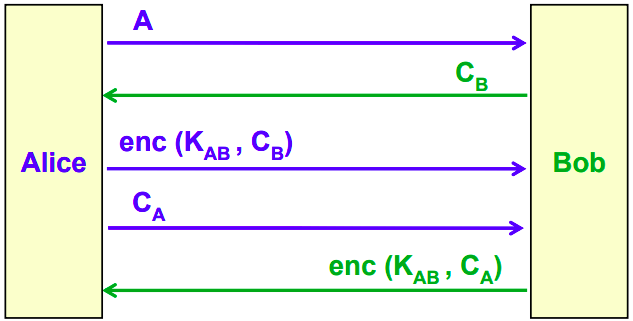
\includegraphics[width=0.7\textwidth]{/home/lorenzo/Notes/Information System Security/images/Screenshot from 2024-11-15 11-52-51.png}
\end{minipage}

\subsubsection{Version 2: Improved Performance}
\begin{minipage}{0.5\textwidth}
    Optimized by reducing the number of messages, which improves performance without compromising security.
    \\ \textbf{Process:}
    \begin{itemize}
        \item Alice includes her identity \((C_A)\) and sends an encrypted challenge (\(C_B)\) in the same message.
        \item Bob responds with his encrypted challenge \(C_A\)to complete the exchange.
    \end{itemize} 

\end{minipage} 
\hspace{0cm}
\begin{minipage}{0.5\textwidth}
    \centering
    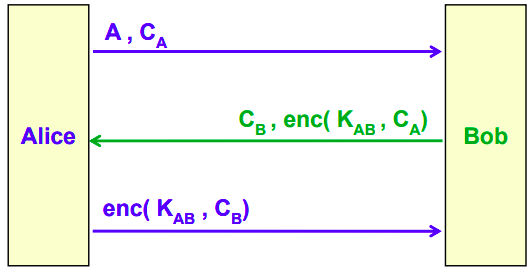
\includegraphics[width=0.7\textwidth]{/home/lorenzo/Notes/Information System Security/images/Screenshot from 2024-11-15 12-04-56.png}
\end{minipage}

%Now I give you some text and I want that you resume it. I don't want many list (this it no means that I don't want there to be any) I want also that you riorganized the sections 
\begin{quotebox}[colframe=blue!10!white, colback=blue!5!white]{Attack on Mutual Symmetric CRA}
    \begin{minipage}{0.5\textwidth}
        \vspace{-0.5cm}
        A potential attacker, "Mike" (posing as Alice), exploits the protocol by mimicking responses:
        \begin{itemize}
            \item The attacker intercepts Alice's identity \((C_A)\) and Bob's challenge \((C_B)\).
            \item The attacker uses the shared key \(K_{AB}\) to manipulate responses and mimic both parties.
        \end{itemize}
    \end{minipage} 
    \hspace{1cm}
    \begin{minipage}{0.3\textwidth}
        \centering
        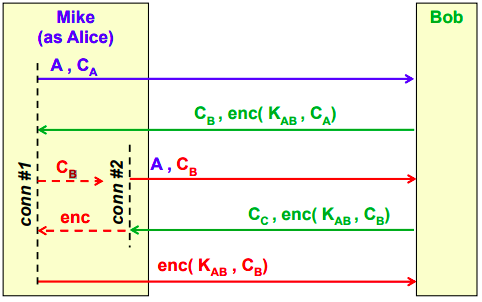
\includegraphics[width=\textwidth]{/home/lorenzo/Notes/Information System Security/images/Screenshot from 2024-11-15 12-09-09.png}
    \end{minipage}
\end{quotebox}

\subsection{Asymmetric CRA}
\begin{minipage}{0.6\textwidth}
%	\vspace{-0.5cm}
    \textbf{Process:}
    \begin{itemize}
        \item A \textbf{random nonce (R)} is generated by the Verifier.
        \item The verifier encrypts \(R\) using the user's public key (\(ID.PK\)) and sends it to the Claimant:
        \(C=enc(ID.PK,R)\)
        \item The Claimant decrypts \(C\) using their private key (\(ID.SK\)) and sends \(R\) back in cleartext:
        \(response=dec(ID.SK,C)\)
        \item The Verifier validates: \(valid(ID)\ \&\&\ (response\ ==\ R)\).
    \end{itemize}
\end{minipage} 
\hspace{0.2cm}
\begin{minipage}{0.4\textwidth}
    \centering
    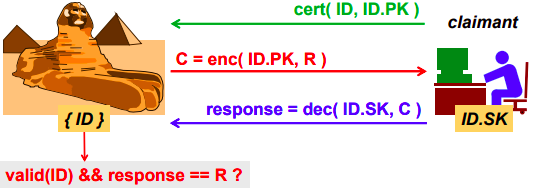
\includegraphics[width=\textwidth]{/home/lorenzo/Notes/Information System Security/images/Screenshot from 2024-11-15 12-43-33.png}
\end{minipage}
\subsubsection{Applications}
\begin{itemize}
    \item  Widely implemented in secure communication protocols like IPsec, SSH, and TLS.
    \item Fundamental in modern authentication frameworks such as FIDO.
\end{itemize}
\begin{quotebox}[colframe=blue!10!white, colback=blue!5!white]{Asymmetric CRA analysis}
    \begin{minipage}{0.5\textwidth}
        \vspace{-1.1cm}
        \subsubsection{Security:}
        \begin{itemize}
            \item It's the strongest mechanism.
            \item Does not require the Verifier to store any shared secret, reducing potential attack vectors.
        \end{itemize}
     \end{minipage} 
     \hspace{0cm}
     \begin{minipage}{0.5\textwidth}
        \subsubsection{Problems:}
        \begin{itemize}
            \item It \textbf{slower} compared to symmetric methods.
            \item If designed inaccurately may lead to an involuntary signature
            by the Claimant.
            \item Trust issues managing root certificates, name constraint, and certificate revocation.
        \end{itemize}
     \end{minipage}
\end{quotebox}

\section{One-Time Password(OTP)}
\begin{minipage}{0.6\textwidth}
\vspace{-1.0cm}
One-Time Passwords are temporary and valid for a single use in an authentication session. They mitigate risks like password reuse and passive sniffing but can still be vulnerable to man-in-the-middle (MITM) attacks. 
These passwords are often designed 
with random characters to prevent 
guessing, but this can make password instertion difficult for users. 
input.
\end{minipage} 
\hspace{0.5cm}
\begin{minipage}{0.4\textwidth}
    
    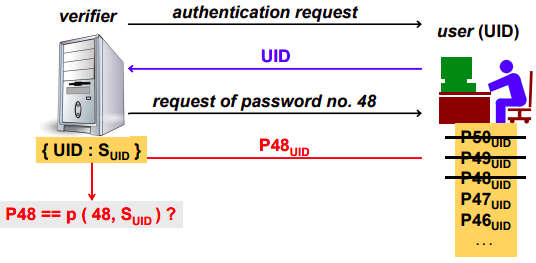
\includegraphics[width=0.8\textwidth]{/home/lorenzo/Notes/Information System Security/images/Screenshot from 2024-11-15 13-11-17.png}
\end{minipage}

\subsection{S/KEY System}
S/KEY System was the first OTP implementation by Bell Labs (1981).
It pre-computes a sequence of passwords derived from a user’s secret. 
Each password is validated and replaced with its predecessor, ensuring security 
without storing the secret:
\[Secret = S_{ID}\]
\[P_1=h(S_{ID}),P_2=h(P_1),...,P_N=h(P_{N-1})\]
\noindent
This approach 
minimizes verifier storage needs and offers robust protection, with users solely 
responsible for password retention.
\subsubsection{One-time generation with S/KEY}

In the S/KEY system, the user creates 
a secret passphrase (PP), which is combined 
with a server-provided seed to generate a 64-bit 
password. The passphrase is concatenated with the seed, 
and an MD4 hash is used to produce the password. 
The result is presented as six short words from a shared 
dictionary, making it easy to remember. This method allows secure password generation while using the same passphrase across multiple servers with different seeds. If the passphrase is compromised, security is at risk.

\chapter{Firewall and IDS/IPS} 

\begin{minipage}{0.6\textwidth}
\section{What is a Firewall?}
%	\vspace{-0.5cm}
A firewall acts as a protective barrier, much like a physical wall against fire. It is primarily a controlled connection point between networks with differing security levels. Its key functions include:
\begin{itemize}
    \item \textbf{Boundary Protection:} Serving as a network filter between trusted (internal) and untrusted (external) networks.
    \item \textbf{Compartmentalization:} Dividing network zones based on security levels to enforce stricter control.
\end{itemize}
\end{minipage} 
\hspace{0.5cm}
\begin{minipage}{0.4\textwidth}
    \centering
    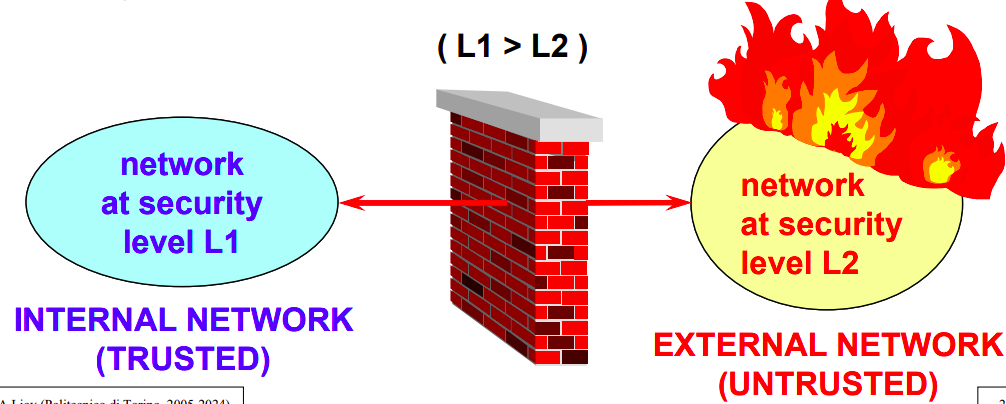
\includegraphics[width=\textwidth]{/home/lorenzo/Notes/Information System Security/images/Screenshot from 2024-11-21 15-09-40.png}
\end{minipage}

\section{Ingress vs Egress firewall}
Firewalls can be classified based on the direction of traffic they manage:
\begin{itemize}
    \item An \textbf{ingress firewall} focuses on incoming connections, typically regulating access to public services provided by the network or supporting exchanges initiated by internal users.
    \item An \textbf{egress firewall} monitors outgoing connections. It's typically used to check the activity of internal personnel [Works well for channel-based services (e.g., TCP applications) but faces challenges with stateless, message-based services (e.g., ICMP, UDP)].
\end{itemize}
\section{The three principles of the firewall}
\begin{enumerate}
    \item The firewall should be the only connection between the internal and external networks.
    \item Only the "authorized"  traffic is allowed to pass the firewall.
    \item The firewall itself must be secure against potential vulnerabilities.
\end{enumerate}
These principles were outlined by \textit{D.Cheswick, S.Bellovin}.

\section{Authorization policies}
\begin{itemize}
    \item \textbf{Permitlist/allowlist}: All that is not explicitly permitted, is forbidden. 
    \begin{itemize}
        \item It offers higher security but it's difficult to manage. 
    \end{itemize}
    \item \textbf{Blocklist/denylist}: All that is not explicitly forbidden, is permitted.
    \begin{itemize}
        \item It's less secure but it's more easy to manage. 
    \end{itemize}
\end{itemize}

\section{Basic components}
Firewalls include several key components that work together to provide security:
\begin{itemize}
    \item \textbf{Packet Filter/ Screening Router / Choke}: Filters traffic at the network level based on packet attributes such as IP headers and transport headers.
    \item \textbf{Bastion Host}: A secure system with auditing capabilities, often positioned to handle critical traffic.
    \item \textbf{Application Gateway (Proxy)}:  Acts on behalf of an application, managing access control and providing detailed packet inspection at the application level.
    \item \textbf{Dual-Homed Gateway}:  A system with two network interfaces and disabled routing, isolating internal and external networks. (In the way we can decide which packets are sent from a network to another).
\end{itemize}

\section{A which level the controls are made?}
Firewalls at higher levels provide more security but tend to be slower, while firewalls at lower levels offer less security but greater speed.
\begin{figure}[h]
    \centering
    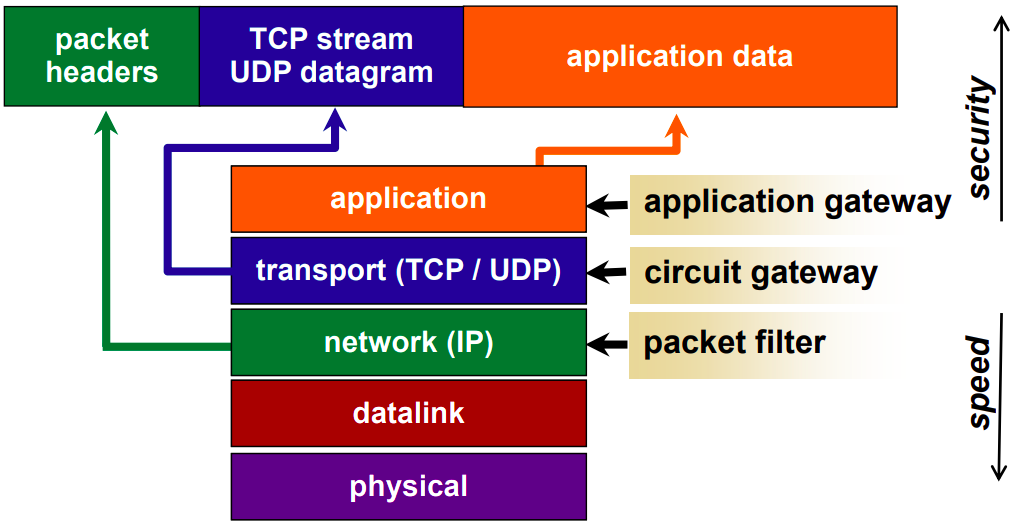
\includegraphics[width=0.5\textwidth]{/home/lorenzo/Notes/Information System Security/images/Screenshot from 2024-11-21 15-43-10.png}
\end{figure}
\begin{quotebox-yellow}{To undersand:}
    \textbf{security is better up} \(\rightarrow\) \textbf{speed is better down}\\
    \textbf{security is better down} \(\rightarrow\) \textbf{speed is better up}
\end{quotebox-yellow}

\section{Network-Level Controls}
Firewalls operate at various levels of the network stack applying different controls based on the type of firewall used:
\begin{itemize}
    \item \textbf{Packet Filters}: Operate at the network level, inspecting packet headers.
    \item \textbf{Stateful Packet Filters}: Track connection states for more dynamic filtering.ù
    \item \textbf{Circuit-Level Gateways / Proxies}: Work at the transport level, ensuring secure connection establishment.
    \item \textbf{Application-Level Gateways / Proxies}: Provide inspection and control at the application layer, often with more granular rules.
\end{itemize}

 \subsection{Packet filter}
 A packet filter inspects packets based on headers, such as IP and transport headers. These filters are traditionally available on routers and now in most OS. They allow for rules like permitting incoming connections to specific services (e.g., a web server) or limiting DNS queries from specific internal servers.

\definecolor{darkgreen}{rgb}{0.0, 0.39, 0.0}  % Custom dark green color
\begin{itemize}
    \item \textcolor{darkgreen}{\textbf{Pro:}} 
    \begin{itemize}
        \item Independent of applications, scalable, and cost-effective (available in many OS and routers).
        \item Good performance and low cost.
    \end{itemize}
    \item \textcolor{red}{\textbf{Cons:}} 
    \begin{itemize}
        \item Vulnerable to attacks like IP spoofing or fragmented packets.
        \item Difficult to support services using dynamically allocated ports (e.g. FTP).
        \item Complex configuration and hard to implement user authentication.
    \end{itemize}
\end{itemize}

\subsection{Circuit-Level Gateway}
A circuit-level gateway acts as a transport-level proxy, creating secure communication channels between client and server without inspecting the payload. It protects against Layer 3/Layer 4 attacks like IP fragmentation or TCP handshake exploits.
\begin{itemize}
    \item \textcolor{darkgreen}{\textbf{Pro:}} 
    \begin{itemize}
        \item Provides protection by isolating the server from attacks.
        \item Offers client authentication and eliminates many low-level attack vectors.
    \end{itemize}
    \item \textcolor{red}{\textbf{Cons:}} 
    \begin{itemize}
        \item Still shares many limitations of packet filters and requires modifications to the application for full functionality.
    \end{itemize}
\end{itemize}

\subsection{Application-Level Gateway}
An application-level gateway (or proxy) operates at the application layer, inspecting the payload of packets. These proxies often require modifications to client applications and can enhance security by checking the semantics of application data (e.g., HTTP methods) or performing peer authentication.
\begin{itemize}
    \item \textcolor{darkgreen}{\textbf{Pro:}} 
    \begin{itemize}
        \item Strong security against application vulnerabilities (e.g., buffer overflow attacks).
        \item Fine-grained access controls and the ability to mask internal IP addresses.
        \item May provide protection against attacks like buffer overflows.
        \item Not transparent to the client and may break the client-server model.
    \end{itemize}
    \item \textcolor{red}{\textbf{Cons:}} 
    \begin{itemize}
        \item Requires specific proxies for each application and can introduce delays when supporting new applications.
        \item High resource usage and lower performance due to user-mode operations.
    \end{itemize}
\end{itemize} 
Variants of application-level proxies include \textbf{transparent proxies}, which are less intrusive to clients, and \textbf{strong application proxies}, which focus on checking data semantics, not just syntax.

\subsection{HTTP Proxies}
An HTTP forward proxy is a server that acts as an intermediary or front-end for client requests. It receives requests from internal users and forwards them to the real external server (So it's a egress control).
\textbf{Benefits:}
\\\vspace{-0.8cm}
\begin{minipage}{0.65\textwidth}
	\vspace{0.5cm}
    \begin{itemize}
        \item \textbf{Shared Cache}: External web pages are cached, reducing load times for all internal users.
        \item \textbf{Authentication and Authorization}: Enforces user authentication and controls access for internal users.
        \item \textbf{Various controls} (e.g. allowed sites, transfer direction, data
        types, …).
    \end{itemize} 
\end{minipage} 
\hspace{0.4cm}
\begin{minipage}{0.3\textwidth}
    \centering
    
\includegraphics[width=1.2\textwidth]{/home/lorenzo/Notes/Information System Security/images/Screenshot from 2024-11-21 17-21-05.png}
\end{minipage}

\begin{quotebox-grey}{Type of Proxies}
    \begin{itemize}
        \item \textbf{Forward Proxy (HTTP Proxy)}: This type of proxy controls outgoing traffic from the internal network to the external one, enforcing access controls and caching content. It provides features like user authentication and authorization, content filtering, and bandwidth control.
        \item \textbf{Reverse Proxy (HTTP Reverse Proxy)}: A reverse proxy sits in front of web servers, providing additional services like load balancing, content inspection, TLS acceleration, and caching. It can obfuscate the internal server structure, improving security, and support performance optimizations like dynamic page feeding based on client speed.
    \end{itemize}
\end{quotebox-grey}

\begin{quotebox}[colframe=blue!10!white, colback=blue!5!white]{Reverse proxy: possibile configuration}
\begin{minipage}{0.5\textwidth}
    \underline{\textbf{Key components:}}
    \begin{itemize}
        \item \textbf{External Network (Red Cloud)}
        \item \textbf{Firewall}
        \item \textbf{DMZ (Demilitarized Zone)}: A buffer zone between external and internal networks where systems that interact with the external network are placed for added security.
        \item \textbf{Reverse Proxy}
        \item \textbf{Internal Network}: The secure area where your actual servers (e.g., serv1, serv2) reside.
    \end{itemize}    
\end{minipage} 
\hspace{0.5cm}
\begin{minipage}{0.45\textwidth}
    \centering
    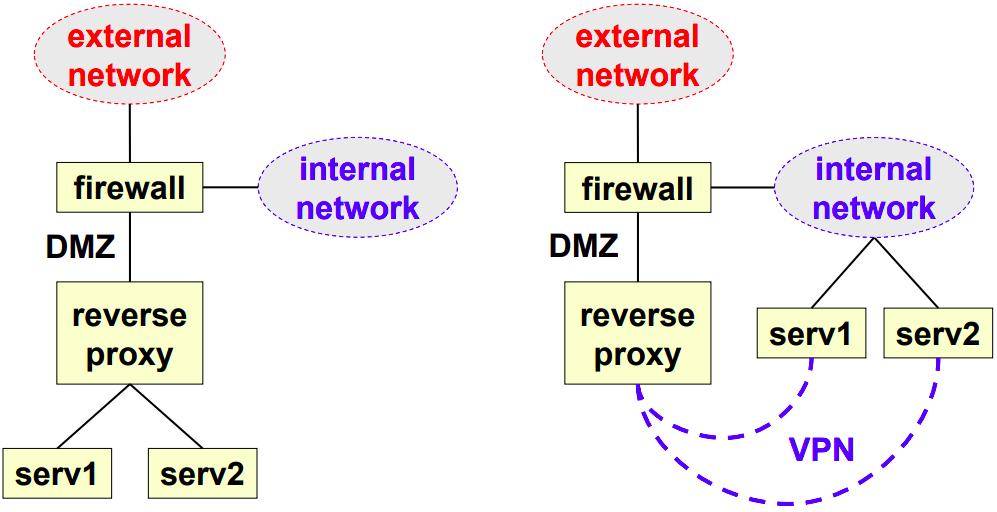
\includegraphics[width=\textwidth]{/home/lorenzo/Notes/Information System Security/images/Screenshot from 2024-11-21 17-38-55.png}
\end{minipage}
\\
\\\\
\underline{\textbf{How configurations work?}}
\\\\
\begin{minipage}[t]{0.45\textwidth}
   \textbf{Left configuration: Direct reverse proxy setup}
   \begin{itemize}
    \item \textbf{Flow:} External user \(\rightarrow\) Reverse Proxy \(\rightarrow\) Internal Servers (serv1, serv2).  
    \item \textbf{Benefits:} Internal servers are hidden and protected, while performance and security are improved.
   \end{itemize}
\end{minipage} 
\hspace{1cm}
\begin{minipage}[t]{0.45\textwidth}
   \textbf{Right Configuration: Reverse Proxy with VPN}
   \begin{itemize}
    \item \textbf{Flow}: External user \(\rightarrow\) Reverse Proxy \(\rightarrow\) Encrypted VPN connection \(\rightarrow\) Internal Servers (serv1, serv2).
    \item \textbf{Benefit}: Adds an extra layer of security through encryption for communication between the reverse proxy and internal servers.
   \end{itemize}
\end{minipage}
\end{quotebox}

\subsection{WAF (Web Application Firewall)}
A WAF is a module installed at a proxy (forward and/or reverse) to filter the application traffic. Filters the followings types of traffic:
\begin{itemize}
    \item HTTP commands.
    \item HTTP request/response headers.
    \item HTTP request/response content.
\end{itemize}
\begin{quotebox-grey}{Popular WAF example: \textbf{ModSecurity}}
    ModSecurity is a widely-used WAF plugin for web servers like Apache and NGINX, offering protection through predefined rules like the OWASP ModSecurity Core Rule Set (CRS).
\end{quotebox-grey}
\section{Firewall's Architectures}
\subsection{"Packet Filter" architecture}
\vspace{0.2cm}
\begin{quotebox-yellow}{What it does?}
This architecture uses a simple packet filter to screen traffic at both the IP and higher protocol levels (like TCP)
\end{quotebox-yellow}
\vspace{0.5cm}
\begin{minipage}{0.5\textwidth}
    \vspace{-0.5cm}
    \textbf{Key Points:}
    \begin{itemize}
        \item If implemented with a router then it's a "screening router" and there's \textbf{no need for extra dedicated hardware}.
        \item The packet filter element represents a \textbf{single point of failure}.
        \item \textbf{There's no need for proxies} or application modifications.
    \end{itemize}
\end{minipage}
\hfill
\begin{minipage}{0.5\textwidth}
    \centering
    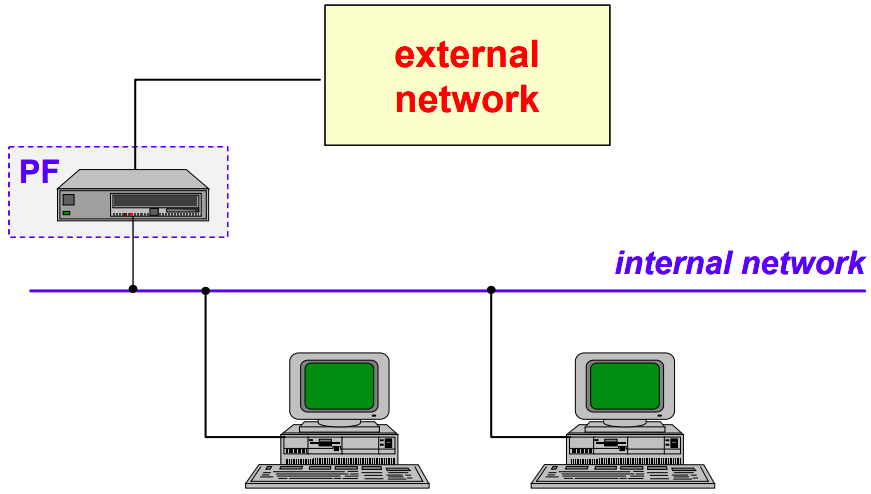
\includegraphics[width=0.8\textwidth]{/home/lorenzo/Notes/Information System Security/images/Screenshot from 2024-11-21 19-10-09.png}
\end{minipage}
\begin{center}
    \begin{quotebox-red}{Beware}
        Simple, cost-effective, but insecure!
        \end{quotebox-red}   
\end{center}
\vspace{0.5cm}
\subsection{"Dual-homed Gateway" architecture}
\vspace{0.2cm}
\begin{quotebox-yellow}{What it does?}
Uses a system with two network interfaces (hence "dual-homed") to provide a basic firewall between external and internal networks.
\end{quotebox-yellow}

\begin{minipage}{0.5\textwidth}
	\vspace{-2cm}
    \textbf{Key Points:}
    \begin{itemize}
        \item Easy to implement with small hardware requirements.
        \item The internal network can be masquerade.
    \end{itemize}
\end{minipage} 
\hfill
\begin{minipage}{0.5\textwidth}
    \centering
    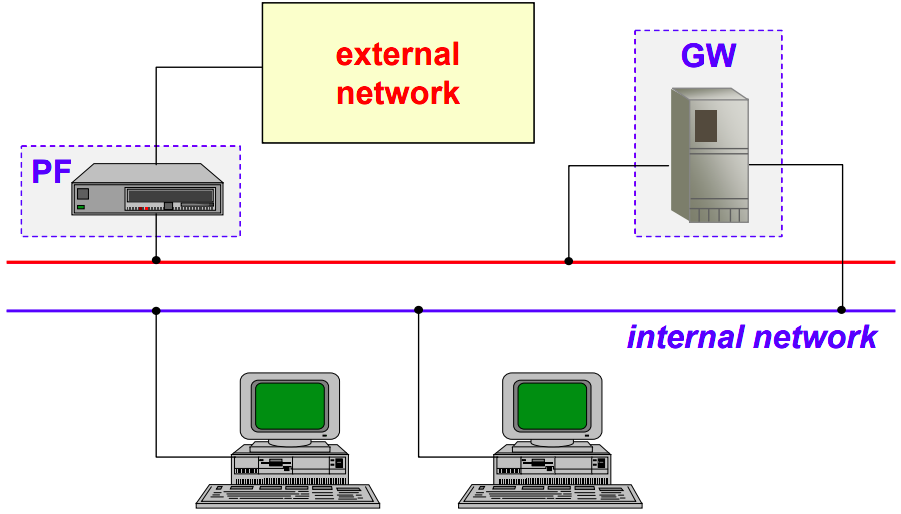
\includegraphics[width=0.8\textwidth]{/home/lorenzo/Notes/Information System Security/images/Screenshot from 2024-11-21 19-41-54.png}
\end{minipage}
\begin{center}
    \begin{quotebox-red}{Beware}
        Inflexible, with higher management overhead and reduced flexibility in handling complex network setups.
    \end{quotebox-red}   
\end{center}

\subsection{"Screened host" architecture}
\vspace{0.2cm}
\begin{quotebox-yellow}{What it does?}
    Uses two primary components: 
    \begin{itemize}
        \item \textbf{Router}
        \item \textbf{Bastion host}
    \end{itemize}
    This setup aims to provide enhanced security by controlling the flow of traffic between the internal and external networks.
\end{quotebox-yellow}

\begin{minipage}{0.5\textwidth}
	\vspace{-1.5cm}
    \textbf{Key Points:}
    \begin{itemize}
        \item Traffic from the internal network (INT) to external (EXT) is blocked unless it’s from the bastion host. Similarly, external traffic is blocked unless directed to the bastion.
        \item More flexible (skip control over some services / hosts)
    \end{itemize}
\end{minipage} 
\hfill
\begin{minipage}{0.5\textwidth}
    \centering
    \includegraphics[width=0.8\textwidth]{
        /home/lorenzo/Pictures/Screenshots/Screenshot from 2024-11-21 21-11-47.png}
\end{minipage}
\begin{center}
    \begin{quotebox-red}{Beware}
        \begin{itemize}
            \item \textbf{More Expensive and Complex} 
       to manage: Requires two systems (router + bastion host) instead of just one.
       \item \textbf{Limited Masking}: Only the host and protocols that go through the bastion host can be masked for security (such as hiding internal IP address or data). However, if the packet filter (PF) uses NAT, it can mask additional traffic and hide internal network details.
     \end{itemize}
    \end{quotebox-red}   
\end{center}

\subsection{"Screened subnet" architecture} 
\vspace{0.2cm}
\begin{quotebox-yellow}{What it does?}
A DMZ (De-Militarized Zone) is created between an internal network and a external network.
The DMZ  acts as a buffer zone to isolate external entities from the internal network, such as web servers or remote access points.
\end{quotebox-yellow}
\begin{minipage}{0.5\textwidth}
	%\vspace{-1.5cm}
    \textbf{Traffic flows:}
    \begin{itemize}
        \item The first firewall controls access from the external network to the DMZ, ensuring only authorized traffic can reach the public-facing systems.
        \item The second firewall restricts traffic from the DMZ to the internal network, allowing only specific and necessary connections.
    \end{itemize}
    \textcolor{darkgreen}{\textbf{It the most secure solution}} \textbf{because this setup hides the internal network from external users, reducing exposure to attacks.}
\end{minipage} 
\hfill
\begin{minipage}{0.5\textwidth}
    \centering
    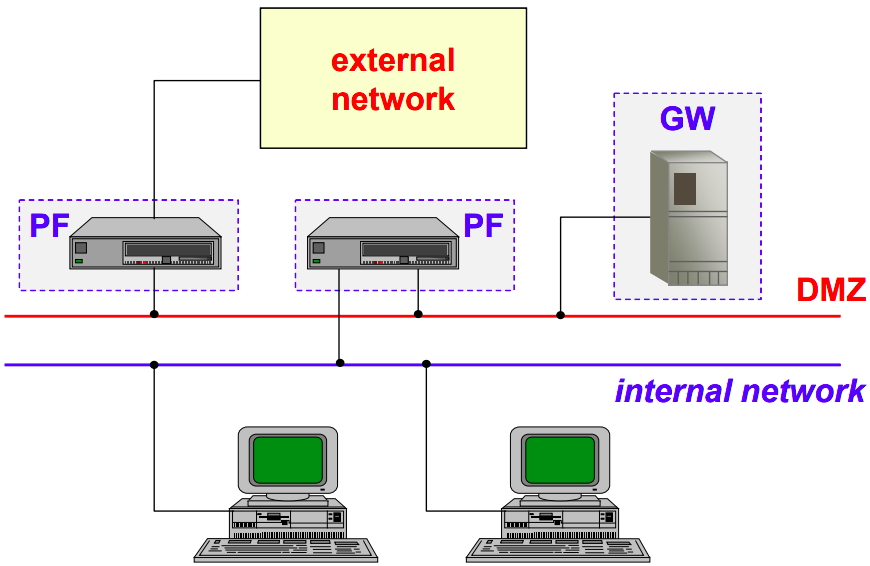
\includegraphics[width=0.8\textwidth]{
        /home/lorenzo/Notes/Information System Security/images/Screenshot from 2024-11-22 10-22-22.png}
\end{minipage}


\begin{center}
    \begin{quotebox-red}{Beware}
      \begin{itemize}
        \item \textbf{Higher cost} due to the additional hardware.
        \item \textbf{The DMZ is home not only to the gateway} but also to other host (typically the public servers).
      \end{itemize} 
    \end{quotebox-red}   
\end{center}
\newpage
\subsection{"Screened subnet" architecture (version 2)}
\vspace{0.2cm}
\begin{quotebox-yellow}{What it does?}
    In this version of the Screened Subnet architecture, the packet filters (\textbf{PF}) and gateway (\textbf{GW}) are merged into a single device that is called \textbf{AKA} ("three-legged firewall").
\end{quotebox-yellow}


\begin{minipage}{0.4\textwidth}
	%\vspace{-1.5cm}
    \textbf{Three-Legged design:}
    \begin{itemize}
        \item One interface connecting to the \textbf{External network} (untrusted).
        \item One interface connecting to the \textbf{Internal network} (trusted).
        \item One interface connecting to the DMZ (where public-facing services reside).
    \end{itemize}
\end{minipage} 
\hfill
\begin{minipage}{0.6\textwidth}
    \centering
    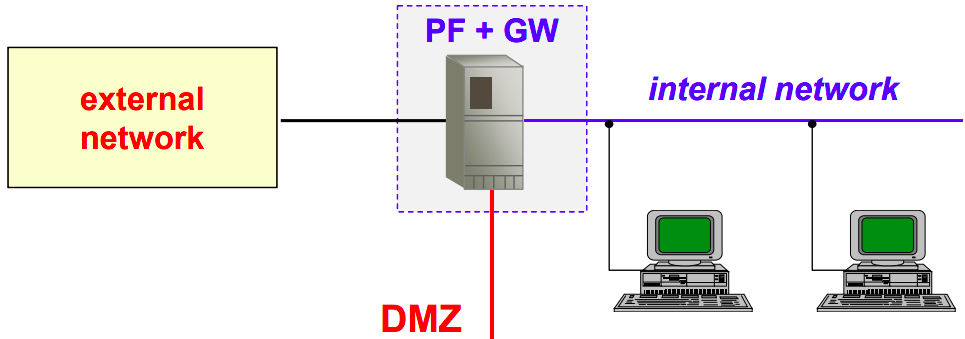
\includegraphics[width=0.8\textwidth]{
        /home/lorenzo/Notes/Information System Security/images/Screenshot from 2024-11-22 10-59-27.png}
\end{minipage}

\begin{center}
    \begin{quotebox-red}{Beware}
      It's \textcolor{darkgreen}{\textbf{more simple}} than the previous version but presents a \textbf{single point of failure}.
    \end{quotebox-red}   
\end{center}
\noindent{\color{gray!50}\rule{\textwidth}{0.5pt}}

\section{Local/Personal Firewall}
This image represents three different firewall configurations: \textbf{Network firewall}, \textbf{Local firewall} and \textbf{Personal firewall}. In the previous pages we have considered the network firewall, now let's start to analyze the Local/Personal firewall. \\
\begin{figure}[h]
    \centering
    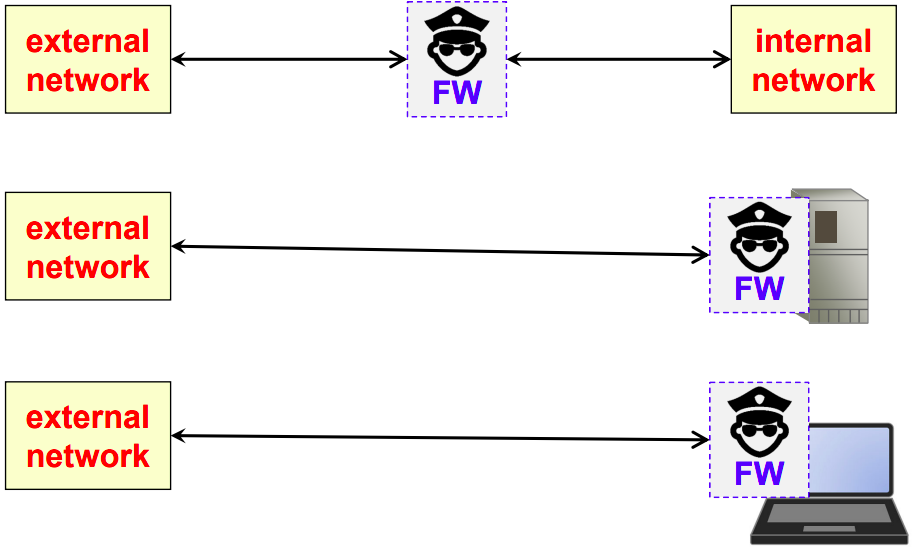
\includegraphics[width=0.5\textwidth]{/home/lorenzo/Notes/Information System Security/images/Screenshot from 2024-11-22 11-51-30.png}
\end{figure}
\\
\noindent
\textbf{A local or personal firewall} is installed directly on a device to protect it from unauthorized access or attacks. Unlike a normal network firewall, it may limit the PROCESSES that are permitted:
\begin{itemize}
    \item To open network channels towards other nodes (client behavior).
    \item To answer network requests (server behavior).
\end{itemize}

\noindent
These features make local firewalls essential for containing malware, blocking trojans, or preventing accidental misconfigurations. \textbf{However, in order to be effective, the firewall management MUST be separated from system management.}

\section{Protection offered by a firewall}
A firewall is 100\% effective only for attacks over/against blocked channels.
The other channels require other protection technique:
\begin{itemize}
    \item \textbf{VPNs}
    \item \textbf{intrusion detection systems (IDS)}
    \item \textbf{application-level protections}
\end{itemize}
\noindent{\color{gray!50}\rule{\textwidth}{0.5pt}}
\section{Intrusion Detection System (IDS)}
\begin{quotebox-yellow}{Definition}
An \textbf{Intrusion Detection System (IDS)}text is a security mechanism designed to:
\begin{itemize}
    \item identify actors using a system or a network without authorization (and their actions).
    \item  identify authorized actors who violate their privileges.
\end{itemize}
\textbf{Hypothesis}
\begin{itemize}
    \item The behavior “pattern” of non-authorized users differs from that of the authorized ones
\end{itemize}
\end{quotebox-yellow}

\subsection{IDS functional features}
\begin{itemize}
    \item \textbf{Passive IDS:} Observes and detects issues but doesn’t act to stop them.\\ \underline{Techniques:}
    \begin{itemize}
        \item Cryptographic checksums to detect changes in files.
        \item Pattern matching to identify attack signatures (e.g., malware signatures).
    \end{itemize}
    \item \textbf{Active IDS:} Monitors activity dynamically and reacts when thresholds are exceeded.\\ \underline{Techniques:}
    \begin{itemize}
        \item Tracks normal behavior to identify anomalies (\textbf{"learning"}).
        \item Gathers detailed statistics on traffic and actions (\textbf{text"monitoring"}).
        \item Triggers alerts or responses when unusual patterns occur (\textbf{"reaction}).
    \end{itemize}
\end{itemize}

\subsection{IDS topological features}
\begin{itemize}
    \item \textbf{HIDS (Host-Based IDS):} Monitors individual devices (hosts).
    \begin{itemize}
        \item Analyzes logs from the OS, services, or applications.
        \item Uses built-in OS tools to track internal activity.
    \end{itemize}
    \item \textbf{NIDS (Network-Based IDS):} Monitors traffic at the network level.
    \item Uses network traffic monitoring tools.
\end{itemize}

\begin{quotebox-grey}{NIDS Architecture}
\underline{\textbf{Components:}}
\begin{itemize}
    \item \textbf{Sensor:} The frontline tool that analyzes traffic or logs looking for suspect patterns. Generates security alerts and can modify access controls (e.g., block traffic).
    \item \textbf{Director:} Coordinates sensors and manages a central database.
    \item \textbf{Message System:}  Ensures secure communication among IDS components.
\end{itemize}
\begin{minipage}{0.5\textwidth}
%	\vspace{-0.5cm}
\underline{\textbf{Workflow:}}
\begin{enumerate}
    \item Traffic from the external network enters through the firewall.
    \item (Net) sensors monitor traffic before it reaches the DMZ or internal network.
    \item Within the DMZ, host sensors monitor server activities.
    \item Traffic entering the internal network is further monitored by both host and network sensors.
    \item All sensors report suspicious activities to the IDS director.
    \item The IDS director consolidates this data and raises alerts or takes action if any patterns of intrusion or policy violations are detected.
\end{enumerate}
\end{minipage} 
\hspace{0.2cm}
\begin{minipage}{0.5\textwidth}
    \centering
    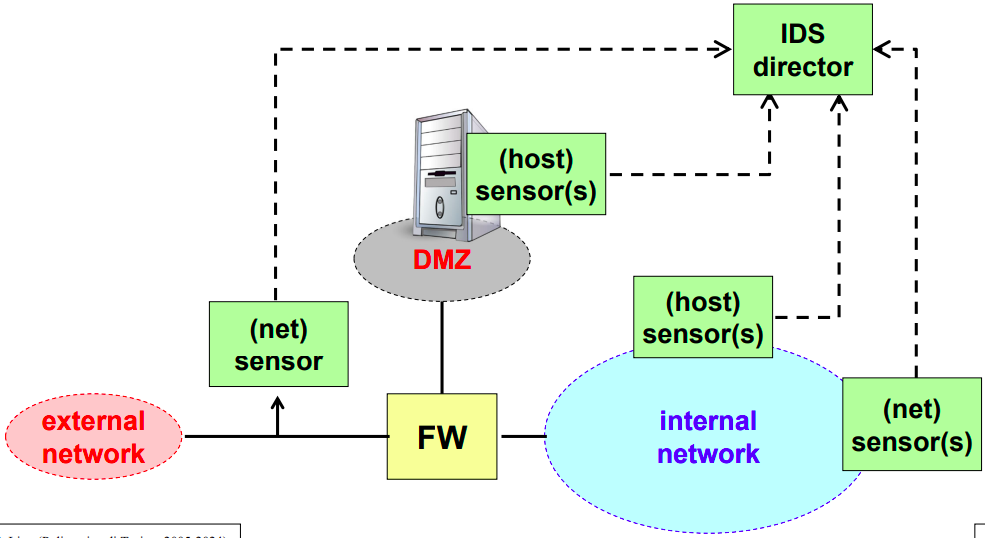
\includegraphics[width=\textwidth]{/home/lorenzo/Pictures/Screenshots/Screenshot from 2024-11-22 14-41-40.png}
\end{minipage}
\end{quotebox-grey}

\section{Intrusion Prevention System (IPS)}
\vspace{0.2cm}
\begin{quotebox-yellow}{Definition}
An \textbf{Intrusion Prevention System (IPS)} is an advanced security technology (not a product) that identifies unauthorized activities like an IDS but actively blocks or mitigates them in real time (= IDS + distributed dynamic firewall).\\ Often, Intrusion Prevention Systems (IPS) are integrated with Intrusion Detection Systems (IDS) into a unified solution called \textbf{Intrusion Detection and Prevention System (IDPS)}
\end{quotebox-yellow}
\noindent
\textcolor{red}{\textbf{N.B.}} IPS requires careful configuration and monitoring to balance its protective capabilities with the risk of blocking innocent traffic.
\begin{center}
\begin{quotebox-red}{Why is it useful to merge IPS with IDS?}
    IPS already has some of IDS's features, such as detection capabilities. But merging IPS with IDS brings many advantages because:
    \begin{itemize}
        \item \textbf{IDS} excels in providing deep visibility into all network activity, including suspicious behavior that might not warrant immediate action.
        \item \textbf{IPS} actively blocks threats, but in doing so, it may not focus as much on monitoring benign-but-suspicious activities.
    \end{itemize}
\end{quotebox-red}
\end{center}











\end{document}